\documentclass[11pt,a4paper]{article}

% Packages;
\usepackage[utf8]{inputenc}
\usepackage[T1]{fontenc}
\usepackage[margin=1in]{geometry}
\usepackage{amsmath,amssymb,amsfonts}
\usepackage{algorithm}
\usepackage{algpseudocode}
\usepackage{booktabs}
\usepackage{longtable}
\usepackage{tabularx}
\usepackage{hyperref}
\usepackage{xcolor}
\usepackage{enumitem}
\usepackage{listings}
\usepackage{graphicx}
\usepackage{float}
\usepackage{parskip}
\usepackage[title]{appendix}
\usepackage{tikz}
\usetikzlibrary{positioning, shapes, arrows}

\hypersetup{
    colorlinks=true,
    linkcolor=blue!70!black,
    citecolor=green!50!black,
    urlcolor=blue!60!black
}

\lstset{
    basicstyle=\ttfamily\small,
    breaklines=true,
    frame=single,
    backgroundcolor=\color{gray!5},
    keywordstyle=\color{blue!70!black},
    commentstyle=\color{green!50!black},
    columns=fullflexible,
}

% Algorithm style tweaks
\algrenewcommand\algorithmicrequire{\textbf{Input:}}
\algrenewcommand\algorithmicensure{\textbf{Output:}}
\algnewcommand\algorithmicforeach{\textbf{for each}}
\algdef{S}[FOR]{ForEach}[1]{\algorithmicforeach\ #1\ \algorithmicdo}

% Title;
\title{Structure Descent: LLM-Guided Discrete Choice Model Specification\\[6pt]
\large Pipeline Documentation and Technical Reference}
\author{}
\date{}

\begin{document}
\maketitle
\tableofcontents
\newpage

%===================================
\section{Changelog; Pipeline Correctness Fixes}
\label{sec:changelog}
%=======================================================================

\textbf{This block supersedes any previously-reported metrics in this document and in downstream notebooks.  Re-run the full pipeline before citing any numbers.}

\begin{description}[style=nextline]

\item[Feature-lookup lookahead leakage (data prep).]
Earlier versions of the notebook pipeline built \texttt{cust\_item\_lookup}, \texttt{cust\_cat\_affinity}, \texttt{cust\_brand\_affinity}, and \texttt{item\_popularity} via \texttt{.groupby(...).last()} / whole-dataframe aggregations.  Because \texttt{.last()} returns the chronologically final state across the \emph{entire} dataframe (train + val + test combined), every event was scored with post-hoc feature values --- a textbook lookahead leak.  Chosen items always had non-null history; random negatives almost always had null (zero) history; the model learned ``pick the non-null item.''

\textbf{The fix}: \texttt{src/data\_prep.py} \texttt{build\_choice\_sets} now attaches a \texttt{chosen\_features} dict to each event populated from the per-row causal columns (\texttt{routine}, \texttt{recency\_days}, \texttt{novelty}, \texttt{cat\_affinity}) that \texttt{compute\_state\_features} already produces via cumcount-style running aggregations.  Notebook cells 7 and 8 now read \texttt{event['chosen\_features']} for positives and apply zero-history defaults for negatives (\texttt{routine=0}, \texttt{recency=1/1000}, \texttt{novelty=1}, \texttt{cat\_affinity=0}, \texttt{brand\_affinity=0}).  \texttt{item\_popularity} is computed from the train split only.

\emph{Consequence:} every previously-reported headline number --- top-1, top-5, MRR, NLL, AIC, BIC, posterior scores, and every baseline's corresponding entry --- is \textbf{stale and inflated}.  All metrics must be re-measured.  Placeholders in this document are tagged \emph{[TODO: rerun post-leakage-fix]}.

\item[{{\texttt{decay}} combinator removed}.]
Layer~3 \texttt{decay(term, halflife)} has been removed entirely from \texttt{src/dsl.py} (\texttt{LAYER3\_COMBINATORS}, \texttt{UNARY\_COMBINATORS}, the \texttt{decay()} function, and the \texttt{compute\_compound\_feature} dispatch branch) and from the outer-loop prompt/annealing schedule in \texttt{src/outer\_loop.py}.  The previous implementation indexed the \emph{transformed} \texttt{recency} score in $[0,1]$ instead of raw days, which made the decay exponent meaningless.  The remaining Layer~3 combinators are \texttt{interaction}, \texttt{split\_by}, \texttt{threshold}, \texttt{log\_transform}, \texttt{ratio}, \texttt{power}, \texttt{difference} (seven total).

\item[Outer-loop \texttt{apply\_proposal} ADD+REMOVE bug.]
Paired ADD~X + REMOVE~Y proposals were falsely rejected because the REMOVE length check was compared against the \emph{original} structure length rather than the post-ADD length.  Net length was unchanged, so the guard bailed.  Fixed in \texttt{src/outer\_loop.py}.

\item[\texttt{\_export\_search\_history} viz bug.]
Rejected/stuck iterations were previously exported as \texttt{accepted\_N} nodes, producing chains of visually identical ``accepted'' nodes whenever proposals were rejected in a row.  Fixed so that only genuinely-accepted iterations emit accepted nodes.

\item[Inner-loop prior kwargs forwarding.]
\texttt{src/inner\_loop.py} \texttt{run\_inner\_loop} now forwards \texttt{**kwargs} ($\sigma$, $\tau$, $\nu$) through to \texttt{compute\_posterior\_score}.

\item[Subsample event weights.]
\texttt{src/subsample.py} \texttt{apply\_subsample} now returns a per-event \texttt{np.ndarray} of length \texttt{len(filtered\_df)} instead of a customer$\to$weight dict.  Notebook cells 4, 10, and 12 now actually thread these weights into \texttt{run\_inner\_loop(event\_weights=...)}.

\end{description}

\subsection{Known Issues and Limitations}

\begin{itemize}
\item \texttt{brand\_affinity} is currently zero for both positives and negatives.  A leakage-safe per-event brand history column is not yet produced in \texttt{compute\_state\_features}.
\item Negative-item \texttt{price} is currently zero.  The negative-sampling path does not join in catalog prices, so \texttt{price\_sensitivity} and \texttt{price\_rank} collapse to the category midpoint for random negatives.
\end{itemize}


%===================================
\section{Data Preparation}
\label{sec:data-prep}
%=======================================================================

\subsection{Amazon Dataset}

\texttt{amazon-purchases.csv}: 1.85 million rows, one row per purchased item.

\begin{table}[H]\centering\tiny
\begin{tabular}{llllll}
\toprule
Date & Price & Qty & State & ASIN & Category \\
\midrule
2018-12-04 & 7.98  & 1 & NJ & B0143RTB1E & FLASH\_MEMORY \\
2018-12-22 & 13.99 & 1 & NJ & B01MA1MJ6H & HEADPHONES \\
2018-12-24 & 8.99  & 1 & NJ & B078JZTFN3 & -- \\
2018-12-25 & 10.45 & 1 & NJ & B06XWF9HML & DISHWARE\_BOWL \\
2018-12-25 & 10.00 & 1 & NJ & B00837ZOI0 & SHAVING\_AGENT \\
\bottomrule
\end{tabular}
\end{table}

Some rows have empty \texttt{Title}/\texttt{Category}.  Rows missing \texttt{customer\_id}/\texttt{order\_date}/\texttt{asin} are removed during data preparation; rows missing only \texttt{category} are kept with category set to \texttt{"Unknown"}.

\texttt{survey.csv} has 5{,}027 respondents across 23 columns, keyed by \texttt{Survey ResponseID}.  Columns fall into three logical groups: Demographics, Amazon usage, and Household/health.  The join model is \texttt{purchases.Survey ResponseID = survey.Survey ResponseID}, many-to-one (each customer has ${\sim}368$ purchases on average).


%---
\subsection{\texttt{load\_data()}; Read Raw CSVs}
%-----------------------------------------------------------------------

Reads the two source files and parses dates.  I/O is isolated so the rest of the pipeline operates on DataFrames.

\begin{algorithm}[H]
\caption{\textsc{LoadData}}\label{alg:load-data}
\begin{algorithmic}[1]
\Require \texttt{purchase\_path}, \texttt{survey\_path}
\Ensure \texttt{(purchases, survey)} DataFrames
\State $\texttt{purchases} \gets \Call{ReadCSV}{\texttt{purchase\_path}, \text{parse ``Order Date'' as datetime}}$
\State $\texttt{survey} \gets \Call{ReadCSV}{\texttt{survey\_path}}$
\State \Return $(\texttt{purchases}, \texttt{survey})$
\end{algorithmic}
\end{algorithm}


%---
\subsection{\texttt{clean\_purchases()}; Normalize and Drop Unusable Rows}
%-----------------------------------------------------------------------

Renames columns to snake\_case, coerces types, drops rows missing \texttt{customer\_id}, \texttt{order\_date}, or \texttt{asin}, fills missing \texttt{category} with \texttt{"Unknown"} and missing \texttt{price} with $0.0$, and sorts by \texttt{(customer\_id, order\_date)}.

\begin{algorithm}[H]
\caption{\textsc{CleanPurchases}}\label{alg:clean-purchases}
\begin{algorithmic}[1]
\Require DataFrame $\texttt{df}$
\Ensure Cleaned, sorted DataFrame
\State Rename columns to snake\_case (e.g.\ ``Order Date'' $\to$ \texttt{order\_date})
\State Parse \texttt{order\_date} as datetime; parse \texttt{price} as float, fill NaN with $0.0$
\State Drop rows where \texttt{customer\_id}, \texttt{order\_date}, or \texttt{asin} is missing
\State Fill missing \texttt{category} with \texttt{"Unknown"}
\State Cast \texttt{customer\_id}, \texttt{asin} to string
\State Sort by $(\texttt{customer\_id}, \texttt{order\_date})$ ascending
\State \Return $\texttt{df}$
\end{algorithmic}
\end{algorithm}


%---
\subsection{\texttt{join\_survey()}; Attach Demographics}
%-----------------------------------------------------------------------

Left-merges \texttt{survey} onto events by \texttt{customer\_id}.

\begin{algorithm}[H]
\caption{\textsc{JoinSurvey}}\label{alg:join-survey}
\begin{algorithmic}[1]
\Require DataFrame $\texttt{df}$, DataFrame $\texttt{survey}$
\Ensure Merged DataFrame
\State Rename survey ``Survey ResponseID'' $\to$ \texttt{customer\_id}
\State Drop all-null columns from \texttt{survey}
\State Snake-case all column names
\State Drop duplicate \texttt{customer\_id}s (keep first)
\State \Return $\texttt{df}.\text{merge}(\texttt{survey}, \text{on}=\texttt{customer\_id}, \text{how}=\text{``left''})$
\end{algorithmic}
\end{algorithm}


%---
\subsection{\texttt{compute\_state\_features()}; Build the Choice State $s_t$}
%-----------------------------------------------------------------------

For each purchase event $t$, compute features summarizing what the customer did \textbf{before} time $t$.  Every feature at row $t$ uses only rows ${<}\,t$ for that customer, so there is no leakage from the future.

\begin{table}[H]\centering\tiny
\begin{tabularx}{\textwidth}{lXX}
\toprule
\textbf{Feature} & \textbf{Computed via} & \textbf{Purpose} \\
\midrule
\texttt{routine} & \texttt{groupby(customer, asin).cumcount()} & Repeat purchase; habit \\
\texttt{novelty} & \texttt{routine == 0} & First-time purchase flag \\
\texttt{recency\_days} & \texttt{order\_date $-$ shift(order\_date)} & Replenishment cycle \\
\texttt{cat\_affinity} & \texttt{groupby(customer, category).cumcount()} & Category taste \\
\texttt{cat\_count\_7d/30d} & Rolling event count & Category momentum \\
\texttt{brand} & Mode first-token; stopword-filtered & Brand identity \\
\bottomrule
\end{tabularx}
\end{table}

\begin{algorithm}[H]
\caption{\textsc{ComputeStateFeatures}}\label{alg:compute-state-features}
\begin{algorithmic}[1]
\Require DataFrame $\texttt{df}$ sorted by $(\texttt{customer\_id}, \texttt{order\_date})$
\Ensure $\texttt{df}$ with state-feature columns appended

\Statex \textit{// Repeat purchases}
\ForEach{$(\texttt{customer\_id}, \texttt{asin})$ group}
    \State \hspace{2em} $\texttt{routine}[i] \gets$ running count of prior rows in this group
\EndFor
\State $\texttt{novelty} \gets \mathbb{1}[\texttt{routine} = 0]$

\Statex \textit{// Recency}
\ForEach{$(\texttt{customer\_id}, \texttt{asin})$ group}
    \State \hspace{2em} $\texttt{last\_date}[i] \gets$ \texttt{order\_date} of previous row in group (\texttt{NaN} if none)
\EndFor
\State $\texttt{recency\_days} \gets (\texttt{order\_date} - \texttt{last\_date})$ in days; fill NaN with 999

\Statex \textit{// Category affinity (cumulative)}
\ForEach{$(\texttt{customer\_id}, \texttt{category})$ group}
    \State \hspace{2em} $\texttt{cat\_affinity}[i] \gets$ running count of prior rows in this group
\EndFor

\Statex \textit{// Time-based category momentum}
\State Sort by $(\texttt{customer\_id}, \texttt{category}, \texttt{order\_date})$
\ForEach{$(\texttt{customer\_id}, \texttt{category})$ group}
    \State \hspace{2em} $\texttt{cat\_count\_7d}[i] \gets$ count of events in the last 7 days (time-based)
    \State \hspace{2em} $\texttt{cat\_count\_30d}[i] \gets$ count of events in the last 30 days
\EndFor
\State Sort back by $(\texttt{customer\_id}, \texttt{order\_date})$

\Statex \textit{// Brand (mode first-token per ASIN; with stopword filter)}
\State Build $\texttt{asin} \to \texttt{brand}$ map from mode of non-stopword first tokens
\State $\texttt{brand}[i] \gets \texttt{brand\_map}[\texttt{asin}[i]]$; collapse singletons $\to$ \texttt{"unknown\_brand"}

\State \Return $\texttt{df}$
\end{algorithmic}
\end{algorithm}


%---
\subsection{\texttt{temporal\_split()}; Per-Customer Train/Val/Test}
%-----------------------------------------------------------------------

For each customer, take their earliest ${\sim}80\%$ of purchases as training, next ${\sim}10\%$ as val, most recent ${\sim}10\%$ as test.

\begin{algorithm}[H]
\caption{\textsc{TemporalSplit}}\label{alg:temporal-split}
\begin{algorithmic}[1]
\Require DataFrame $\texttt{df}$; $\texttt{val\_frac}=0.1$; $\texttt{test\_frac}=0.1$
\Ensure $\texttt{df}$ with \texttt{"split"} column added
\State Sort $\texttt{df}$ by $(\texttt{customer\_id}, \texttt{order\_date})$
\ForEach{customer group of size $n$}
    \State \hspace{2em} $n_{\text{test}} \gets \max(1, \lfloor n \cdot \texttt{test\_frac} \rfloor)$
    \State \hspace{2em} $n_{\text{val}} \gets \max(1, \lfloor n \cdot \texttt{val\_frac} \rfloor)$
    \If{$n_{\text{test}} + n_{\text{val}} \ge n$}
        \State \hspace{2em} \hspace{2em} $n_{\text{test}}, n_{\text{val}} \gets 1, 0$ \Comment{tiny-customer fallback}
    \EndIf
    \State \hspace{2em} $n_{\text{train}} \gets n - n_{\text{val}} - n_{\text{test}}$
    \State \hspace{2em} Label first $n_{\text{train}}$ rows $\to$ \texttt{"train"}; next $n_{\text{val}} \to$ \texttt{"val"}; last $n_{\text{test}} \to$ \texttt{"test"}
\EndFor
\State \Return $\texttt{df}$
\end{algorithmic}
\end{algorithm}


%---
\subsection{\texttt{attach\_train\_popularity()}; Split-Aware Popularity}
%-----------------------------------------------------------------------

\begin{algorithm}[H]
\caption{\textsc{AttachTrainPopularity}}\label{alg:attach-pop}
\begin{algorithmic}[1]
\Require DataFrame $\texttt{df}$ with \texttt{"split"} column
\State \hspace{2em} $\texttt{pop}[\texttt{asin}] \gets$ count of rows where $\texttt{split} = \texttt{"train"}$; grouped by \texttt{asin}
\State \hspace{2em} $\texttt{df.popularity} \gets \texttt{df.asin}.\text{map}(\texttt{pop}).\text{fillna}(0)$
\State \Return $\texttt{df}$
\end{algorithmic}
\end{algorithm}


%---
\subsection{\texttt{build\_choice\_sets()}; Assemble (Positive, Negatives) Per Event}
\label{sec:build-choice-sets}
%-----------------------------------------------------------------------

Conditional logit needs; for every observed purchase; a set of alternatives the customer \emph{could have chosen instead}.  Each event's choice set is approximated as the true purchase + 9 sampled negatives; half same-category (hard negatives); half random (easy negatives; popularity-weighted).

\begin{algorithm}[H]
\caption{\textsc{BuildChoiceSets}}\label{alg:build-choice-sets}
\begin{algorithmic}[1]
\Require DataFrame $\texttt{df}$, $n_{\text{neg}}=9$, $\texttt{seed}=42$, $n_{\text{resamples}}=1$
\Ensure List of choice-set records
\State $\texttt{catalog} \gets$ unique ASINs in $\texttt{df}$
\State $\texttt{first\_seen}[\texttt{asin}] \gets$ earliest \texttt{order\_date} per ASIN
\State $\texttt{pop}[\texttt{asin}] \gets \texttt{df.popularity}$ \Comment{train-only}
\State Sort \texttt{catalog} by \texttt{first\_seen}
\State $\texttt{records} \gets []$

\ForEach{event row $r = (\texttt{customer}, \texttt{date}, \texttt{asin}=\texttt{chosen}, \texttt{category}, \ldots)$}
    \State $\texttt{avail} \gets \{a \in \texttt{catalog} : \texttt{first\_seen}[a] < \texttt{date}\}$ \Comment{strict $<$}
    \For{$k = 0$ \textbf{to} $n_{\text{resamples}} - 1$}
        \State $\texttt{rng}_k \gets$ deterministic RNG seeded from $(\texttt{seed}, k, \texttt{event\_index})$
        \If{$\texttt{category} = \texttt{"Unknown"}$}
            \State $\texttt{negs} \gets$ sample $n_{\text{neg}}$ from $\texttt{avail}$, weighted by $\texttt{pop}$
        \Else
            \State $\texttt{same\_cat} \gets \{a \in \texttt{avail} : \texttt{category}[a] = \texttt{category},\; a \ne \texttt{chosen}\}$
            \State $\texttt{neg\_cat} \gets$ sample $\lfloor n_{\text{neg}}/2 \rfloor$ from \texttt{same\_cat}, weighted by $\texttt{pop}$
            \State $\texttt{neg\_rand} \gets$ sample $(n_{\text{neg}} - \lfloor n_{\text{neg}}/2 \rfloor)$ from $\texttt{avail}$, weighted by $\texttt{pop}$
            \State $\texttt{negs} \gets \texttt{neg\_cat} \mathbin\Vert \texttt{neg\_rand}$
        \EndIf
        \State $\texttt{choices} \gets \text{shuffle}([\texttt{chosen}] \mathbin\Vert \texttt{negs})$
        \State $\texttt{chosen\_idx} \gets$ position of \texttt{chosen} in \texttt{choices}
    \EndFor

    \Statex \textit{// Leakage-safe: snapshot current row's causal columns}
    \State $\texttt{chosen\_features} \gets \{\texttt{routine}: r.\texttt{routine},\; \texttt{recency\_days}: r.\texttt{recency\_days},$
    \Statex \hspace{8em} $\texttt{novelty}: r.\texttt{novelty},\; \texttt{cat\_affinity}: r.\texttt{cat\_affinity}, \ldots\}$
    \State Append record to $\texttt{records}$
\EndFor
\State \Return $\texttt{records}$
\end{algorithmic}
\end{algorithm}

\subsection{Data Prep Pipeline Summary}

\begin{lstlisting}[frame=none,backgroundcolor=\color{white}]
load_data -> clean_purchases -> join_survey -> compute_state_features
  -> filter customers with >= 5 purchases -> temporal_split
  -> attach_train_popularity -> [optional subsample] -> build_choice_sets
\end{lstlisting}

After this, each training instance is a tuple $(s_t, \mathcal{A}_t, a^*_t)$: the customer's state at time $t$, the 10-item candidate set, and the observed pick.

%=======================================================================
\section{\texttt{src/dsl.py} --- Feature Grammar}
\label{sec:dsl}
%=======================================================================

The DSL defines what transformations of the state $s_t$ are legal to write into the utility function:
\[
u_\theta(a, s) = \sum_{k=1}^{|S|} \theta_k \cdot \text{term}_k(a, s)
\]
The inner loop fits the $\theta_k$ for a given $S$; the outer loop (LLM) proposes new $S$.

\begin{table}[H]\centering\tiny
\begin{tabularx}{\textwidth}{lXX}
\toprule
\textbf{Layer} & \textbf{Purpose} & \textbf{Examples} \\
\midrule
1. Universal primitives & Behavioral signals for any domain & \texttt{routine}; \texttt{recency}; \texttt{novelty}; \texttt{popularity} \\
2. Amazon-specific & Domain-specific e-commerce signals & \texttt{price\_sensitivity}; \texttt{rating\_signal}; \texttt{brand\_affinity} \\
3. Combinators & Build new terms from existing ones & \texttt{interaction}; \texttt{split\_by}; \texttt{threshold}; \texttt{log\_transform}; \texttt{ratio}; \texttt{power}; \texttt{difference} \\
\bottomrule
\end{tabularx}
\end{table}

\subsection{DSLTerm and DSLStructure}

A \texttt{DSLTerm} is either \textbf{simple} (a base-column reference, e.g.\ \texttt{routine}) or \textbf{compound} (a combinator applied to base terms, e.g.\ \texttt{interaction(routine, recency)}).

A \texttt{DSLStructure} is an ordered bag of terms. Key properties:
\begin{itemize}
\item $\text{complexity}(S) = L(S)$: simple terms cost 1, compound terms cost $1 + |\text{args}|$.
\item $\log p(S) = -L(S) \cdot \ln 2$ --- the prior pressure against big structures.
\item $\texttt{initial}() \to S = [\texttt{routine}, \texttt{affinity}]$.
\end{itemize}

\subsection{\texttt{compute\_compound\_feature}}

\begin{algorithm}[H]
\caption{\textsc{ComputeCompoundFeature}}\label{alg:compute-compound}
\begin{algorithmic}[1]
\Require \texttt{term} (DSLTerm); \texttt{base\_features} (dict; name $\to$ array)
\Ensure Computed feature array
\If{\texttt{term.name} = \texttt{"interaction"}}
    \State \hspace{2em} \Return $\texttt{base\_features}[\texttt{args}[0]] \times \texttt{base\_features}[\texttt{args}[1]]$
\ElsIf{\texttt{term.name} = \texttt{"split\_by"}}
    \State \hspace{2em} \Return $\Call{SplitBy}{\texttt{base\_features}[\texttt{args}[0]], \texttt{base\_features}[\texttt{args}[1]]}$
\ElsIf{\texttt{term.name} = \texttt{"difference"}}
    \State \hspace{2em} \Return $\texttt{base\_features}[\texttt{args}[0]] - \texttt{base\_features}[\texttt{args}[1]]$
\ElsIf{\texttt{term.name} = \texttt{"ratio"}}
    \State \hspace{2em} \Return $\Call{Ratio}{\texttt{base\_features}[\texttt{args}[0]], \texttt{base\_features}[\texttt{args}[1]]}$
\ElsIf{\texttt{term.name} = \texttt{"log\_transform"}}
    \State \hspace{2em} \Return $\Call{LogTransform}{\texttt{base\_features}[\texttt{args}[0]]}$
\ElsIf{\texttt{term.name} = \texttt{"power"}}
    \State \hspace{2em} \Return $\Call{Power}{\texttt{base\_features}[\texttt{args}[0]], \texttt{term.kwargs}[\texttt{"exponent"}]}$
\ElsIf{\texttt{term.name} = \texttt{"threshold"}}
    \State \hspace{2em} \Return $\Call{Threshold}{\texttt{base\_features}[\texttt{args}[0]], \texttt{term.kwargs}[\texttt{"cutoff"}]}$
\Else
    \State \hspace{2em} \textbf{raise} ``unknown combinator''
\EndIf
\end{algorithmic}
\end{algorithm}

\subsection{\texttt{build\_structure\_features}}

\begin{algorithm}[H]
\caption{\textsc{BuildStructureFeatures}}\label{alg:build-struct-feats}
\begin{algorithmic}[1]
\Require \texttt{structure}, $\texttt{full\_base\_features} \in \mathbb{R}^{n_{\text{alts}} \times n_{\text{base}}}$, \texttt{all\_term\_names}
\Ensure Feature matrix $\in \mathbb{R}^{n_{\text{alts}} \times |S|}$
\State $\texttt{term\_to\_idx} \gets$ map each base term name to column index
\State $\texttt{columns} \gets []$
\ForEach{term in \texttt{structure.terms}}
    \If{term is simple}
        \State $\texttt{idx} \gets \texttt{term\_to\_idx}[\texttt{term.name}]$
        \State Append $\texttt{full\_base\_features}[:, \texttt{idx}]$ to $\texttt{columns}$
    \Else
        \State $\texttt{base\_dict} \gets \{\text{name}: \texttt{full\_base\_features}[:, i] \mid (\text{name}, i) \in \texttt{term\_to\_idx}\}$
        \State $\texttt{col} \gets \Call{ComputeCompoundFeature}{\texttt{term}, \texttt{base\_dict}}$
        \State Append $\texttt{col}$ to $\texttt{columns}$
    \EndIf
\EndFor
\State \Return $\Call{ColumnStack}{\texttt{columns}}$
\end{algorithmic}
\end{algorithm}


%===================================
\section{\texttt{src/subsample.py}; Leverage-Score Customer Subsampling}
\label{sec:subsample}
%=======================================================================

\subsection{Goal}

Leverage-score sampling picks customers whose behavior profiles are most informative, clusters them to guarantee coverage across behavior types, and attaches importance weights so the subsample's objective approximates the full-data objective in expectation.

The customer profile matrix is $X \in \mathbb{R}^{n_{\text{customers}} \times d}$.

\subsection{\texttt{build\_customer\_profiles()}}

\begin{algorithm}[H]
\caption{\textsc{BuildCustomerProfiles}}\label{alg:build-profiles}
\begin{algorithmic}[1]
\Require DataFrame $\texttt{df}$; $n_{\text{pca}} = 20$
\Ensure $(\texttt{profiles\_df}, X \in \mathbb{R}^{n \times d})$
\State \hspace{2em} $\texttt{cat\_counts} \gets$ pivot table (rows=customer; cols=category; values=count; fill=0)
\State \hspace{2em} $\texttt{cat\_fracs}[i] \gets \texttt{cat\_counts}[i] / \sum \texttt{cat\_counts}[i]$
\State \hspace{2em} $\texttt{cat\_pca} \gets \Call{PCA}{n_{\text{pca}}}.\text{fit\_transform}(\texttt{cat\_fracs})$
\ForEach{customer $c$}
    \State \hspace{2em} \hspace{2em} $\texttt{repeat\_rate}[c] \gets \text{mean}(\mathbb{1}[\texttt{routine} > 0])$
    \State \hspace{2em} \hspace{2em} $\texttt{mean\_recency}[c] \gets \text{mean}(1 / (1 + \texttt{recency\_days}))$
    \State \hspace{2em} \hspace{2em} $\texttt{novelty\_rate}[c] \gets \text{mean}(\mathbb{1}[\texttt{novelty} = 1])$
    \State \hspace{2em} \hspace{2em} $\texttt{purchase\_freq}[c] \gets \log(1 + \texttt{total\_events})$
    \State \hspace{2em} \hspace{2em} $\texttt{cat\_entropy}[c] \gets -\sum_k p_k \log p_k$
\EndFor
\State \hspace{2em} $\texttt{profiles} \gets \Call{Concat}{\texttt{cat\_pca}, \text{scalar features}}$
\State \hspace{2em} $X \gets (\texttt{profiles} - \mu) / \sigma$ \Comment{standardize each column}
\State \Return $(\texttt{profiles\_df}, X)$
\end{algorithmic}
\end{algorithm}

\subsection{\texttt{compute\_leverage\_scores()}}

\begin{algorithm}[H]
\caption{\textsc{ComputeLeverageScores}}\label{alg:leverage}
\begin{algorithmic}[1]
\Require $X \in \mathbb{R}^{n \times d}$
\Ensure Leverage scores $h \in \mathbb{R}^n$
\State $U, S, V^\top \gets \Call{ThinSVD}{X}$
\State $\texttt{mask} \gets (S > 10^{-6})$
\State $U_{\text{eff}} \gets U[:, \texttt{mask}]$
\State $h_i \gets \sum_j U_{\text{eff}}[i, j]^2$ \Comment{row-wise squared norm}
\State \Return $h$
\end{algorithmic}
\end{algorithm}

\subsection{\texttt{subsample\_customers()}}

\begin{algorithm}[H]
\caption{\textsc{SubsampleCustomers}}\label{alg:subsample}
\begin{algorithmic}[1]
\Require DataFrame $\texttt{df}$, $n_{\text{cust}}=500$, $\texttt{min\_per\_cluster}=2$, $\texttt{seed}=42$
\Ensure $(\texttt{selected\_ids}, \texttt{weights})$
\State $\texttt{rng} \gets$ seeded RNG
\State $(\texttt{profiles\_df}, X) \gets \Call{BuildCustomerProfiles}{\texttt{df}}$
\State $h \gets \Call{ComputeLeverageScores}{X}$; clip $h \ge 10^{-10}$

\Statex \textit{// K-Means clustering}
\State $n_{\text{clusters}} \gets \text{clip}(n_{\text{cust}} / 5, \; 2, \; n_{\text{total}})$
\State $\texttt{labels} \gets \Call{KMeans}{n_{\text{clusters}}, \texttt{seed}}.\text{fit\_predict}(X)$

\Statex \textit{// Phase A: top-leverage per cluster (guaranteed coverage)}
\State $\texttt{selected} \gets \emptyset$
\For{$k = 0$ \textbf{to} $n_{\text{clusters}} - 1$}
    \State $\texttt{members} \gets \{i : \texttt{labels}[i] = k\}$, sorted by $h$ descending
    \State $\texttt{selected} \gets \texttt{selected} \cup \texttt{members}[:\texttt{min\_per\_cluster}]$
\EndFor

\Statex \textit{// Phase B: fill remaining budget by leverage-proportional sampling}
\State $\texttt{budget} \gets n_{\text{cust}} - |\texttt{selected}|$
\If{$\texttt{budget} > 0$}
    \State $\texttt{candidates} \gets \text{all indices} \setminus \texttt{selected}$
    \State $\texttt{probs} \gets h[\texttt{candidates}] / \sum h[\texttt{candidates}]$
    \State $\texttt{chosen} \gets \texttt{rng.choice}(\texttt{candidates}, \texttt{budget}, \text{replace}=\text{False}, p=\texttt{probs})$
    \State $\texttt{selected} \gets \texttt{selected} \cup \texttt{chosen}$
\EndIf

\Statex \textit{// Importance weights}
\State $p_i^{\text{eff}} \gets h[\texttt{selected}] / \sum h$
\State $w_i^{\text{raw}} \gets 1 / (n_{\text{cust}} \cdot p_i^{\text{eff}})$
\State $w_i \gets w_i^{\text{raw}} \cdot (n_{\text{total}} / \sum w^{\text{raw}})$ \Comment{normalize so $\sum w_i = n_{\text{total}}$}
\State \Return $(\texttt{selected\_ids}, w)$
\end{algorithmic}
\end{algorithm}

\subsection{\texttt{apply\_subsample()}}

\begin{algorithm}[H]
\caption{\textsc{ApplySubsample}}\label{alg:apply-sub}
\begin{algorithmic}[1]
\Require $\texttt{df}$, $\texttt{selected\_ids}$, $\texttt{weights}$
\Ensure $(\texttt{filtered\_df}, \texttt{event\_weights} \in \mathbb{R}^{|\texttt{filtered\_df}|})$
\State $\texttt{weight\_by\_customer} \gets \text{dict}(\text{zip}(\texttt{selected\_ids}, \texttt{weights}))$
\State $\texttt{filtered\_df} \gets \texttt{df}[\texttt{customer\_id} \in \texttt{selected\_ids}]$
\State $\texttt{event\_weights} \gets [w[\texttt{cid}] \text{ for } \texttt{cid} \in \texttt{filtered\_df.customer\_id}]$
\State \Return $(\texttt{filtered\_df}, \texttt{event\_weights})$
\end{algorithmic}
\end{algorithm}


%===================================
\section{\texttt{src/inner\_loop.py}}
\label{sec:inner-loop}
%=======================================================================

\subsection{Hierarchical Weight Decomposition}

Per-customer, per-category weights:
\[
\theta_{i,c} = \underbrace{\theta_g}_{\text{global}} + \underbrace{\theta_c}_{\text{category offset}} + \underbrace{\delta_i}_{\text{individual offset}}
\]

\begin{table}[H]\centering
\begin{tabular}{lccc}
\toprule
Component & Prior std & Penalty $1/\text{std}^2$ & Effective claim \\
\midrule
$\theta_g$ & $\sigma = 10$  & $0.01$ & ``nearly unconstrained'' \\
$\theta_c$ & $\tau = 1$     & $1$    & ``moderate deviation'' \\
$\delta_i$ & $\nu = 0.5$    & $4$    & ``close to category mean'' \\
\bottomrule
\end{tabular}
\end{table}

\subsection{MAP Estimation Objective}

\[
J(\theta) = -\sum_t w_t \log P_\theta(a^*_t \mid \mathcal{A}_t) + \frac{\|\theta_g\|^2}{2\sigma^2} + \frac{1}{2\tau^2}\sum_c \|\theta_c\|^2 + \frac{1}{2\nu^2}\sum_i \|\delta_i\|^2
\]

\subsection{\texttt{fit\_weights()}}

\begin{algorithm}[H]
\caption{\textsc{FitWeights}}\label{alg:fit-weights}
\begin{algorithmic}[1]
\Require \texttt{structure}, \texttt{features\_list}, \texttt{chosen\_indices}, \texttt{customer\_ids}, \texttt{categories}, $\sigma{=}10$, $\tau{=}1$, $\nu{=}0.5$, \texttt{event\_weights}
\Ensure \texttt{HierarchicalWeights}
\State $n_T \gets |\texttt{structure.terms}|$
\State $\texttt{unique\_cats}, \texttt{unique\_custs} \gets$ sorted unique categories / customers
\State $n_C \gets |\texttt{unique\_cats}|$; \; $n_I \gets |\texttt{unique\_custs}|$
\State Build index maps: $\texttt{cat\_idx}$, $\texttt{cust\_idx}$
\State $\texttt{total\_params} \gets n_T \cdot (1 + n_C + n_I)$
\State $\texttt{ew} \gets$ \texttt{event\_weights} if provided, else all-ones

\Statex
\Function{Unpack}{$x$}
    \State $\theta_g \gets x[: n_T]$
    \State $\theta_c \gets \text{reshape}(x[n_T : n_T + n_C \cdot n_T],\; [n_C, n_T])$
    \State $\delta_i \gets \text{reshape}(x[n_T + n_C \cdot n_T :],\; [n_I, n_T])$
    \State \Return $(\theta_g, \theta_c, \delta_i)$
\EndFunction

\Statex
\Function{Objective}{$x$}
    \State $(\theta_g, \theta_c, \delta_i) \gets \Call{Unpack}{x}$
    \State $\texttt{nll} \gets 0$
    \ForEach{event $e$}
        \State $w \gets \theta_g + \theta_c[\texttt{cat\_idx}[\texttt{cat}_e]] + \delta_i[\texttt{cust\_idx}[\texttt{cid}_e]]$
        \State $\texttt{utilities} \gets \texttt{feats}_e \cdot w$
        \State $\texttt{nll} \mathrel{{-}{=}} \texttt{ew}[e] \cdot \text{log\_softmax}(\texttt{utilities})[\texttt{chosen}_e]$
    \EndFor
    \State $\texttt{reg} \gets \|\theta_g\|^2 / (2\sigma^2) + \|\theta_c\|^2 / (2\tau^2) + \|\delta_i\|^2 / (2\nu^2)$
    \State \Return $\texttt{nll} + \texttt{reg}$
\EndFunction

\Statex
\State $\texttt{result} \gets \Call{Minimize}{\textsc{Objective},\; x_0 = \mathbf{0},\; \text{L-BFGS-B},\; \text{maxiter}=500}$
\State $(\theta_g, \theta_c, \delta_i) \gets \Call{Unpack}{\texttt{result}.x}$
\State \Return $\textsc{HierarchicalWeights}(\theta_g, \theta_c, \delta_i)$
\end{algorithmic}
\end{algorithm}


\subsection{\texttt{compute\_posterior\_score()}}

\begin{algorithm}[H]
\caption{\textsc{ComputePosteriorScore}}\label{alg:posterior-score}
\begin{algorithmic}[1]
\Require \texttt{structure}, \texttt{weights}, \texttt{features\_list}, \texttt{chosen\_indices}, \texttt{customer\_ids}, \texttt{categories}, $\sigma$, $\tau$, $\nu$, \texttt{event\_weights}
\Ensure Scalar score
\State $\texttt{ew} \gets$ \texttt{event\_weights} if provided, else all-ones
\State $\texttt{log\_lik} \gets 0$
\ForEach{event $e$}
    \State $w \gets \texttt{weights}.\text{get\_weights}(\texttt{cid}_e, \texttt{cat}_e)$
    \State $\texttt{log\_lik} \mathrel{{+}{=}} \texttt{ew}[e] \cdot \text{log\_softmax}(\texttt{feats}_e \cdot w)[\texttt{chosen}_e]$
\EndFor
\State $\log p(\theta) \gets -\|\theta_g\|^2 / (2\sigma^2) - \sum_c \|\theta_c\|^2 / (2\tau^2) - \sum_i \|\delta_i\|^2 / (2\nu^2)$
\State $\log p(S) \gets \texttt{structure}.\text{log\_prior}()$ \Comment{$= -L(S) \cdot \ln 2$}
\State \Return $\texttt{log\_lik} + \log p(\theta) + \log p(S)$
\end{algorithmic}
\end{algorithm}

\subsection{\texttt{run\_inner\_loop()}}

\begin{algorithm}[H]
\caption{\textsc{RunInnerLoop}}\label{alg:run-inner}
\begin{algorithmic}[1]
\Require \texttt{structure}, \texttt{features\_list}, \texttt{chosen\_indices}, \texttt{customer\_ids}, \texttt{categories}, \texttt{event\_weights}, \texttt{**kwargs}
\Ensure $(\texttt{weights}, \texttt{score})$
\State $\texttt{weights} \gets \Call{FitWeights}{\texttt{structure}, \ldots, \texttt{event\_weights}, \texttt{**kwargs}}$
\State $\texttt{score} \gets \Call{ComputePosteriorScore}{\texttt{structure}, \texttt{weights}, \ldots, \texttt{event\_weights}}$
\State \Return $(\texttt{weights}, \texttt{score})$
\end{algorithmic}
\end{algorithm}


\subsection{\texttt{fit\_weights\_no\_hierarchy()}}

Ablation baseline with a single flat weight vector $\theta_g$.

\begin{algorithm}[H]
\caption{\textsc{FitWeightsNoHierarchy}}\label{alg:fit-flat}
\begin{algorithmic}[1]
\Require \texttt{structure}, \texttt{features\_list}, \texttt{chosen\_indices}, $\sigma{=}10$, \texttt{event\_weights}
\Ensure $\hat\theta \in \mathbb{R}^{|S|}$
\State $\texttt{ew} \gets$ \texttt{event\_weights} if provided, else all-ones
\Function{Objective}{$x$}
    \State $\texttt{nll} \gets \sum_e -\texttt{ew}[e] \cdot \text{log\_softmax}(\texttt{feats}_e \cdot x)[\texttt{chosen}_e]$
    \State \Return $\texttt{nll} + \|x\|^2 / (2\sigma^2)$
\EndFunction
\State $\texttt{result} \gets \Call{Minimize}{\textsc{Objective}, x_0 = \mathbf{0}, \text{method}=\text{L-BFGS-B}}$
\State \Return $\texttt{result}.x$
\end{algorithmic}
\end{algorithm}


%===================================
\section{\texttt{src/outer\_loop.py}; LLM-Driven Structure Search}
\label{sec:outer-loop}
%=======================================================================

\subsection{Annealing Schedule}

\begin{table}[H]\centering
\begin{tabular}{ll}
\toprule
Iterations & Allowed operations \\
\midrule
0--1 & ADD / REMOVE on Layer~1/2 base terms only \\
2--3 & + \texttt{interaction} and \texttt{split\_by} combinators \\
4+   & All combinators \\
\bottomrule
\end{tabular}
\end{table}

\subsection{Accept Strategies}

\subsubsection{Greedy}
Accept iff $\text{score}_{\text{new}} > \text{score}_{\text{current}}$.

\subsubsection{Simulated Annealing (Metropolis--Hastings)}
\[
P(\text{accept}) = \exp(\Delta / T_i), \quad \Delta = \text{score}_{\text{new}} - \text{score}_{\text{current}}, \quad T_i = T_{\text{start}} + (T_{\text{end}} - T_{\text{start}}) \cdot \frac{i}{n_{\text{iter}}}
\]

\subsubsection{Threshold Accepting}
Accept iff $\Delta > -\tau_i$, where $\tau_i$ shrinks linearly from $\tau_{\text{start}}$ to $\tau_{\text{end}}$.

\subsubsection{Late Acceptance Hill Climbing}
Accept iff $\text{score}_{\text{new}} > \texttt{buffer}[\text{oldest}]$, where $\texttt{buffer}$ is a circular buffer of the last $L$ accepted scores.


\subsection{Outer Loop --- High-Level Pseudocode}

\begin{algorithm}[H]
\caption{\textsc{RunStructureDescent}}\label{alg:outer-loop}
\begin{algorithmic}[1]
\Require $S_0$, \texttt{fit\_fn}, \texttt{get\_metrics\_fn}, \texttt{get\_residuals\_fn}, $n_{\text{iter}}$, \texttt{accept\_strategy}, \texttt{checkpoint}
\Ensure \texttt{history}
\State $(S, \texttt{score}, \texttt{history}, \texttt{proposal\_log}, i_0) \gets \Call{InitOrResume}{S_0, \texttt{fit\_fn}, \texttt{checkpoint}}$
\State $\texttt{weights} \gets \texttt{fit\_fn}(S).\texttt{weights}$
\For{$i = i_0$ \textbf{to} $n_{\text{iter}}$}
    \Statex \textit{// 1. Diagnostics}
    \State $\texttt{metrics} \gets \texttt{get\_metrics\_fn}(\texttt{weights}, S)$
    \State $\texttt{residuals} \gets \texttt{get\_residuals\_fn}(\texttt{weights}, S)$
    \State $\texttt{report} \gets \Call{GenerateDiagnostics}{S, \texttt{score}, \texttt{metrics}, \texttt{residuals}, \ldots}$
    \Statex \textit{// 2. Ask the LLM}
    \State $\texttt{proposal} \gets \Call{PromptLLM}{\texttt{report}, i}$ \Comment{may throw}
    \Statex \textit{// 3. Validate + apply}
    \State $S' \gets \Call{ApplyProposal}{S, \texttt{proposal}}$
    \If{$S' = \texttt{None}$ or $S'.\texttt{terms} = S.\texttt{terms}$} \textbf{continue} \EndIf
    \Statex \textit{// 4. Inner loop}
    \State $(\_,\; \texttt{new\_score}) \gets \texttt{fit\_fn}(S')$
    \State $\Delta \gets \texttt{new\_score} - \texttt{score}$
    \Statex \textit{// 5. Accept / reject}
    \If{$\texttt{accept\_strategy}.\text{decide}(\texttt{score}, \texttt{new\_score}, i, n_{\text{iter}})$}
        \State $S, \texttt{score} \gets S', \texttt{new\_score}$
        \State $(\texttt{weights}, \texttt{score}) \gets \texttt{fit\_fn}(S)$
    \EndIf
    \Statex \textit{// 6. Log + checkpoint}
    \State Append to \texttt{proposal\_log} and \texttt{history}; save checkpoint
\EndFor
\State \Return \texttt{history}
\end{algorithmic}
\end{algorithm}


%=======================================================================
\section{Evaluation Metrics}
\label{sec:eval}
%=======================================================================

\subsection{Notation}
$E$ = held-out events, $J = 10$ alternatives, $c_e$ = chosen index, $s_{e,j}$ = utility score, $p_{e,j} = \text{softmax}(s_{e,\cdot})_j$.

\subsection{Rank Convention}
\[
r_e = |\{j \in \{0, \ldots, J-1\} : s_{e,j} > s_{e,c_e}\}| \qquad \text{(strict $>$; ties favour the chosen)}
\]

\subsection{Predictive Accuracy Metrics}
\begin{align}
\text{top-1} &= \frac{1}{E} \sum_{e=1}^{E} \mathbb{1}[r_e = 0] \\
\text{top-5} &= \frac{1}{E} \sum_{e=1}^{E} \mathbb{1}[r_e < 5] \\
\text{MRR}   &= \frac{1}{E} \sum_{e=1}^{E} \frac{1}{r_e + 1}
\end{align}

\subsection{Negative Log-Likelihood}
\[
\text{NLL} = -\frac{1}{E} \sum_{e=1}^{E} \log \frac{\exp(s_{e,c_e})}{\sum_{j=0}^{J-1} \exp(s_{e,j})}
\]

\subsection{Information Criteria}
\[
\text{AIC} = 2k + 2\,n_{\text{train}} \cdot \text{NLL}_{\text{test}}, \qquad
\text{BIC} = k \log \max(n_{\text{train}}, 2) + 2\,n_{\text{train}} \cdot \text{NLL}_{\text{test}}
\]

These use the test NLL but scale by $n_{\text{train}}$ --- a deliberate project-specific convention yielding a generalization-aware information criterion.

\subsection{\texttt{compute\_metrics()}}

\begin{algorithm}[H]
\caption{\textsc{ComputeMetrics}}\label{alg:compute-metrics}
\begin{algorithmic}[1]
\Require \texttt{features\_list}, \texttt{chosen\_indices}, \texttt{weight\_fn}, \texttt{customer\_ids}, \texttt{categories}
\Ensure Metrics dict
\State $\texttt{top1}, \texttt{top5} \gets 0, 0$; \; $\texttt{rr\_list} \gets []$; \; $\texttt{nll\_sum} \gets 0$; \; $E \gets |\texttt{features\_list}|$
\ForEach{$(\texttt{feats}, c_e, \texttt{cid}, \texttt{cat})$}
    \State $w \gets \texttt{weight\_fn}(\texttt{cid}, \texttt{cat})$
    \State $s \gets \texttt{feats} \cdot w$; \; $p \gets \text{softmax}(s)$
    \State $r_e \gets |\{j : s[j] > s[c_e]\}|$
    \State $\texttt{top1} \mathrel{{+}{=}} \mathbb{1}[r_e = 0]$; \; $\texttt{top5} \mathrel{{+}{=}} \mathbb{1}[r_e < 5]$
    \State Append $1/(r_e + 1)$ to $\texttt{rr\_list}$
    \State $\texttt{nll\_sum} \mathrel{{-}{=}} \log(p[c_e] + 10^{-12})$
\EndFor
\State \Return $\{\texttt{top1}: \texttt{top1}/E,\; \texttt{top5}: \texttt{top5}/E,\; \texttt{mrr}: \text{mean}(\texttt{rr\_list}),\; \texttt{val\_nll}: \texttt{nll\_sum}/E\}$
\end{algorithmic}
\end{algorithm}

\subsection{Stratified Breakdowns}

Four stratified breakdowns slice test events into groups and report per-group top-1:
\begin{enumerate}
\item \textbf{By category}: top-1 and NLL per product category.
\item \textbf{By repeat vs.\ novel}: split by whether the chosen item was previously purchased.
\item \textbf{By activity level}: low/medium/high tertiles by customer purchase count.
\item \textbf{By time of day}: morning (6--12), afternoon (12--18), evening (18--23), night (23--6).
\end{enumerate}


%=======================================================================
\section{Baseline Evaluation Harness}
\label{sec:baselines-harness}
%=======================================================================

\subsection{\texttt{FittedBaseline} Protocol}

Every baseline must implement:
\begin{itemize}
\item \texttt{score\_events(batch)} $\to$ list of per-alternative utility arrays
\item \texttt{n\_params} $\to$ effective parameter count
\item \texttt{description} $\to$ human-readable one-liner
\end{itemize}

\subsection{\texttt{evaluate\_baseline()}}

\begin{algorithm}[H]
\caption{\textsc{EvaluateBaseline}}\label{alg:eval-baseline}
\begin{algorithmic}[1]
\Require \texttt{fitted} (FittedBaseline), \texttt{batch} (BaselineEventBatch), $n_{\text{train}}$, \texttt{fit\_time}
\Ensure \texttt{BaselineReport}
\State $\texttt{scores\_list} \gets \texttt{fitted}.\text{score\_events}(\texttt{batch})$
\State $n \gets |\texttt{scores\_list}|$; assert $n = \texttt{batch}.n_{\text{events}}$
\State $\texttt{top1}, \texttt{top5} \gets 0, 0$; \; $\texttt{rr\_list} \gets []$; \; $\texttt{total\_nll} \gets 0$
\State Initialize $\texttt{per\_cat}$, $\texttt{per\_bucket}$ accumulators
\ForEach{$(\texttt{scores}, \texttt{chosen}, \texttt{cat}, \texttt{meta})$}
    \State $\texttt{probs} \gets \text{softmax}(\texttt{scores})$
    \State $\texttt{rank} \gets |\{j : \texttt{scores}[j] > \texttt{scores}[\texttt{chosen}]\}|$
    \State $\texttt{correct} \gets \mathbb{1}[\texttt{rank} = 0]$
    \State Update $\texttt{top1}$, $\texttt{top5}$, $\texttt{rr\_list}$, $\texttt{total\_nll}$
    \State Update $\texttt{per\_cat}[\texttt{cat}]$, $\texttt{per\_bucket}$
\EndFor
\State $\overline{\text{NLL}} \gets \texttt{total\_nll} / n$
\State $k \gets \max(\texttt{fitted}.n_{\text{params}}, 1)$
\State $\text{AIC} \gets 2k + 2 \cdot n_{\text{train}} \cdot \overline{\text{NLL}}$
\State $\text{BIC} \gets \log(\max(n_{\text{train}}, 2)) \cdot k + 2 \cdot n_{\text{train}} \cdot \overline{\text{NLL}}$
\State \Return $\Call{BaselineReport}{\texttt{top1}/n, \texttt{top5}/n, \text{mean}(\texttt{rr\_list}), \overline{\text{NLL}}, \text{AIC}, \text{BIC}, \ldots}$
\end{algorithmic}
\end{algorithm}

\subsection{\texttt{n\_params} Conventions}

\begin{table}[H]\centering\small
\begin{tabularx}{\textwidth}{lX}
\toprule
Family & Convention \\
\midrule
LASSO-MNL, Bayesian ARD        & count of non-zero coefficients after shrinkage \\
Random Forest, Gradient Boosting & total leaf count across all trees \\
MLP                              & total scalar weight count (incl.\ biases) \\
Paz VNS, Delphos, Structure Descent & $n_{\text{terms}} \cdot (1 + n_{\text{cats}} + n_{\text{custs}})$ \\
DUET                             & $F$ (linear) + neural branch weight+bias count \\
\bottomrule
\end{tabularx}
\end{table}


%=======================================================================
\section{Feature Pool (\texttt{src/baselines/feature\_pool.py})}
\label{sec:feature-pool}
%=======================================================================

The four expansion blocks for the 102-dimensional pool ($d = 12$ base features):

\begin{table}[H]\centering
\begin{tabular}{lll}
\toprule
Block & Formula & Count \\
\midrule
Identity            & $x_i$                                       & $d = 12$ \\
Signed log1p        & $\text{sign}(x_i) \cdot \log(1 + |x_i|)$   & $d = 12$ \\
Signed square       & $\text{sign}(x_i) \cdot x_i^2$              & $d = 12$ \\
Pairwise interactions & $x_i \cdot x_j,\; i < j$                  & $\binom{d}{2} = 66$ \\
\midrule
\textbf{Total}      &                                              & $D = 102$ \\
\bottomrule
\end{tabular}
\end{table}

\subsection{\texttt{build\_expanded\_pool()}}

\begin{algorithm}[H]
\caption{\textsc{BuildExpandedPool}}\label{alg:expand-pool}
\begin{algorithmic}[1]
\Require $\texttt{base\_feats} \in \mathbb{R}^{n_{\text{alts}} \times n_{\text{base}}}$, \texttt{base\_names}, \texttt{include\_interactions}
\Ensure $(\texttt{expanded} \in \mathbb{R}^{n_{\text{alts}} \times D}, \texttt{names})$
\State $\texttt{columns} \gets []$; \; $\texttt{names} \gets []$
\ForEach{$i, \texttt{nm}$ in enumerate(\texttt{base\_names})} \Comment{Identity}
    \State Append $\texttt{base\_feats}[:, i]$; append \texttt{nm}
\EndFor
\ForEach{$i, \texttt{nm}$ in enumerate(\texttt{base\_names})} \Comment{Signed log1p}
    \State $x \gets \texttt{base\_feats}[:, i]$
    \State Append $\text{sign}(x) \cdot \log(1 + |x|)$; append \texttt{"log1p\_"} + \texttt{nm}
\EndFor
\ForEach{$i, \texttt{nm}$ in enumerate(\texttt{base\_names})} \Comment{Signed square}
    \State Append $\text{sign}(x) \cdot x^2$; append \texttt{"sq\_"} + \texttt{nm}
\EndFor
\If{\texttt{include\_interactions}} \Comment{Pairwise}
    \For{$i = 0$ \textbf{to} $n_{\text{base}} - 1$}
        \For{$j = i + 1$ \textbf{to} $n_{\text{base}} - 1$}
            \State Append $\texttt{base\_feats}[:, i] \times \texttt{base\_feats}[:, j]$
        \EndFor
    \EndFor
\EndIf
\State \Return $(\Call{ColumnStack}{\texttt{columns}}, \texttt{names})$
\end{algorithmic}
\end{algorithm}


%=======================================================================
\section{LASSO-MNL (\texttt{src/baselines/lasso\_mnl.py})}
\label{sec:lasso}
%=======================================================================

\subsection{Objective}

\[
\mathcal{L}(\mathbf{w}; \alpha) = \sum_{e=1}^{E} \bigl[-\log \text{softmax}(\mathbf{X}_e \mathbf{w})[c_e]\bigr] + \alpha \|\mathbf{w}\|_1
\]

Gradient of the smooth part:
\[
\nabla_{\mathbf{w}} f(\mathbf{w}) = \sum_{e=1}^{E} \mathbf{X}_e^\top (\mathbf{p}_e - \mathbf{e}_{c_e})
\]

\subsection{Fitting procedure}

The implementation uses FISTA (Fast Iterative Shrinkage-Thresholding Algorithm) with adaptive backtracking line search to solve the inner optimization problem.  The outer loop employs a warm-started path: penalties are sorted from largest (most shrinkage) to smallest, and the solution from one $\alpha$ initializes the next, reducing computation time.  The fitted model uses a hard threshold ($|w_j| < 10^{-6} \to w_j = 0$) to promote sparsity.


%=======================================================================
\section{Bayesian ARD (\texttt{src/baselines/bayesian\_ard.py})}
\label{sec:ard}
%=======================================================================

\subsection{Prior Structure}

\[
\alpha_j \sim \text{Gamma}(a_0, b_0), \qquad w_j \mid \alpha_j \sim \mathcal{N}\!\left(0, \frac{1}{\alpha_j}\right), \qquad j = 1, \ldots, D
\]

\subsection{Joint Posterior}

\[
p(\mathbf{w}, \boldsymbol{\alpha} \mid \mathcal{D}) \propto \left[\prod_{e=1}^{E} p(c_e \mid \mathbf{X}_e, \mathbf{w})\right] \cdot \prod_{j=1}^{D} \mathcal{N}(w_j; 0, 1/\alpha_j) \cdot \prod_{j=1}^{D} \text{Gamma}(\alpha_j; a_0, b_0)
\]

\subsection{Fitting procedure}

The model is implemented in NumPyro and uses Hamiltonian MCMC (NUTS) for posterior inference.  Prior hyperparameters are set to $a_0 = b_0 = 10^{-3}$ (weakly informative).  Inference runs for 500 warmup and 500 post-warmup samples.  Posterior means are extracted per coefficient, and a hard threshold ($|\hat{w}_j| < 10^{-2} \to w_j = 0$) is applied for interpretability.


%=======================================================================
\section{Classical ML Baselines (\texttt{src/baselines/classical\_ml.py})}
\label{sec:classical-ml}
%=======================================================================

\subsection{Binary Classification Adaptation}

Each event is flattened into $J$ rows with binary label $y_{e,j} = \mathbb{1}[j = c_e]$.  At prediction time, scores are $s_{e,j} = \log \mathbb{P}(Y = 1 \mid \mathbf{x}_{e,j})$.

All three baselines use uniform per-row sample weight $w_{e,j} = 1/J$ (not \texttt{class\_weight="balanced"}) to preserve calibration.

\subsection{RandomForestChoice}
Bagging of decision trees.  $k_{\text{RF}} = \sum_{t=1}^{T} n_{\text{leaves}}(t)$.

\subsection{GradientBoostingChoice}
Histogram-based gradient boosting.  $k_{\text{GB}} = \sum_{m=1}^{M} n_{\text{leaves}}(\text{tree}_m)$.

\subsection{MLPChoice}
Two hidden layers $(32, 16)$ with ReLU, wrapped in a \texttt{Pipeline(StandardScaler, MLPClassifier)}.  $k_{\text{MLP}} = \sum_\ell (n_{\ell-1} \cdot n_\ell + n_\ell)$.  Does \emph{not} receive \texttt{sample\_weight} (sklearn limitation).


%=======================================================================
\section{Paz VNS (\texttt{src/baselines/paz\_vns.py})}
\label{sec:paz-vns}
%=======================================================================

\subsection{Multi-Objective Formulation}

Each candidate $S$ is scored on two minimized objectives:
\[
f(S) = \bigl(\text{BIC}(S),\; -\overline{\rho^2_{\text{adj}}}(S)\bigr)
\]

\subsection{Search procedure}

VNS optimizes a two-objective Pareto front: BIC (model complexity) and negative adjusted pseudo-$R^2$ (fit quality).  The algorithm operates in three phases: (1) \emph{Shake}, a random perturbation of the current structure proportional to a neighborhood radius $k$; (2) \emph{Local Improvement}, a first-improvement greedy search over N1 (single ADD/REMOVE) and N2 (random two-step) neighbors up to an evaluation budget; (3) \emph{Archive}, updating the Pareto front with the improved solution.  The radius $k$ resets to 1 on success and increments on failure, implementing the classic VNS strategy.  Restarts from the Pareto front prevent premature convergence.


%=======================================================================
\section{DUET ANN (\texttt{src/baselines/duet\_ga.py})}
\label{sec:duet}
%=======================================================================

\subsection{Utility and Loss}

\[
u(x_{ia} \mid \beta, \theta) = \beta^\top x_{ia} + f_\theta(x_{ia})
\]

Training minimizes:
\[
\mathcal{L}(\beta, \theta) = \underbrace{-\frac{1}{|B|}\sum_{i \in B} \log P_i(c_i)}_{\text{NLL}} + \underbrace{\ell_2 \|\theta\|_2^2}_{\text{MLP L2}} + \underbrace{\lambda_{\text{mono}} \sum_{j \in \mathcal{M}} \text{mean}_{i,a}\bigl[\max(0, -s_j \partial_{x_j} u)\bigr]^2}_{\text{soft monotonicity}}
\]

\subsection{Hybrid architecture and training}

DUET combines a linear component ($\beta$) with a neural network ($f_\theta$), trained end-to-end via gradient descent.  Domain constraints are incorporated via a soft monotonicity penalty: for each feature $j$ flagged as monotonic increasing (sign $s_j$), the term $\max(0, -s_j \partial_{x_j} u)^2$ is penalized, encouraging gradients to align with domain expectations without enforcing them strictly.  The penalty is computed via automatic differentiation with second-order gradient tracking.  Training uses Adam with early stopping on validation NLL and a patience counter.


%=======================================================================
\section{Delphos (\texttt{src/baselines/delphos.py})}
\label{sec:delphos}
%=======================================================================

Delphos (Nova, Hess \& van Cranenburgh, 2025) frames specification as an MDP solved by a Deep Q-Network.

\subsection{Deep Q-Network-based search}

DQN optimizes a policy for sequential structure modifications. Episodes are generated via $\epsilon$-greedy sampling over available actions (ADD/REMOVE terms). At episode termination, an \emph{estimator bridge} evaluates the final structure, producing a scalar reward (e.g., $-\text{BIC}$, or negative NLL).  Rewards are back-propagated exponentially into earlier steps via the Bellman update to encourage good long-horizon choices. The target network is periodically hard-copied from the policy network for learning stability, and $\epsilon$ decays linearly over episodes.  Experience from all episodes is stored in a replay buffer and used for mini-batch gradient updates against the Bellman target.


%=======================================================================
\section{Architecture and Pipeline Overview}
\label{sec:architecture}
%=======================================================================

\subsection{Data Preparation Pipeline}

The data flows through seven sequential stages:

\begin{center}
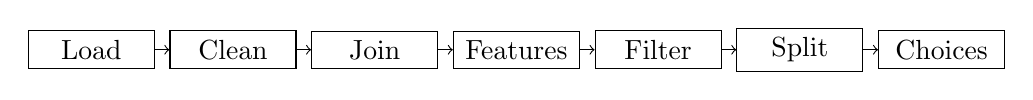
\begin{tikzpicture}[node distance=1.8cm, auto]
  \node (load) [draw, rectangle, minimum width=1.6cm] {Load};
  \node (clean) [draw, rectangle, right of=load, minimum width=1.6cm] {Clean};
  \node (join) [draw, rectangle, right of=clean, minimum width=1.6cm] {Join};
  \node (features) [draw, rectangle, right of=join, minimum width=1.6cm] {Features};
  \node (filter) [draw, rectangle, right of=features, minimum width=1.6cm] {Filter};
  \node (split) [draw, rectangle, right of=filter, minimum width=1.6cm] {Split};
  \node (choice) [draw, rectangle, right of=split, minimum width=1.6cm] {Choices};

  \draw [->] (load) -- (clean);
  \draw [->] (clean) -- (join);
  \draw [->] (join) -- (features);
  \draw [->] (features) -- (filter);
  \draw [->] (filter) -- (split);
  \draw [->] (split) -- (choice);
\end{tikzpicture}
\end{center}

\textbf{Outputs}: $(s_t, \mathcal{A}_t, a^*_t)$ tuples for each purchase event.

\subsection{Structure Descent Architecture}

Structure discovery alternates between two loops:

\begin{center}
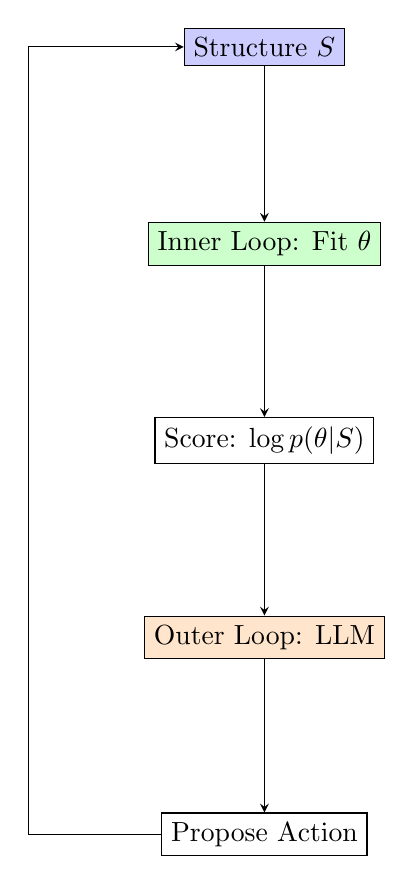
\begin{tikzpicture}[node distance=2.5cm, auto, >={stealth}]
  \node (structure) [draw, rectangle, fill=blue!20] {Structure $S$};
  \node (inner) [draw, rectangle, fill=green!20, below of=structure] {Inner Loop: Fit $\theta$};
  \node (score) [draw, rectangle, below of=inner] {Score: $\log p(\theta|S)$};
  \node (outer) [draw, rectangle, fill=orange!20, below of=score] {Outer Loop: LLM};
  \node (llmcall) [draw, rectangle, below of=outer] {Propose Action};
  
  \draw [->] (structure) -- (inner);
  \draw [->] (inner) -- (score);
  \draw [->] (score) -- (outer);
  \draw [->] (outer) -- (llmcall);
  \draw [->] (llmcall) -- +(-3, 0) |- (structure);
\end{tikzpicture}
\end{center}

\textbf{Inner Loop}: Fits $\theta$ via hierarchical MAP estimation; outputs posterior score.

\textbf{Outer Loop}: LLM reads diagnostics; proposes ADD/REMOVE/MODIFY actions; accepts via strategy.

\subsection{DSL Three-Layer Hierarchy}

\begin{center}
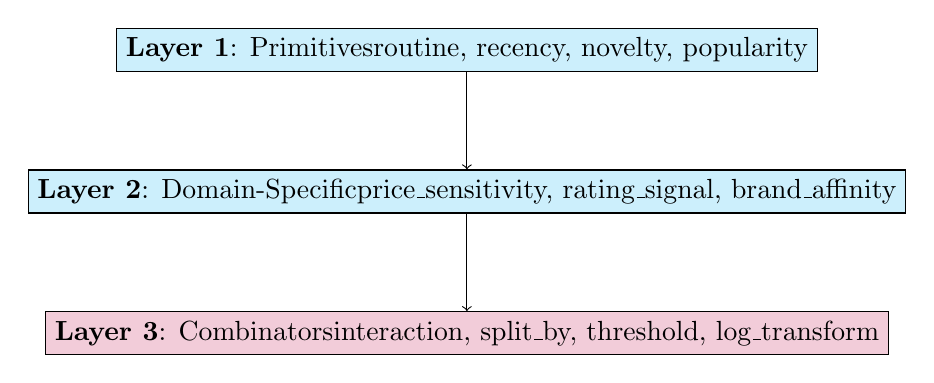
\begin{tikzpicture}[node distance=1.8cm, auto]
  \node (layer1) [draw, rectangle, fill=cyan!20, minimum width=5cm] {
    \textbf{Layer 1}: Primitives \\
    routine, recency, novelty, popularity
  };
  
  \node (layer2) [draw, rectangle, fill=cyan!20, below of=layer1, minimum width=5cm] {
    \textbf{Layer 2}: Domain-Specific \\
    price\_sensitivity, rating\_signal, brand\_affinity
  };
  
  \node (layer3) [draw, rectangle, fill=purple!20, below of=layer2, minimum width=5cm] {
    \textbf{Layer 3}: Combinators \\
    interaction, split\_by, threshold, log\_transform
  };
  
  \draw [->] (layer1) -- (layer2);
  \draw [->] (layer2) -- (layer3);
\end{tikzpicture}
\end{center}

All layers compose into utility: $u = \sum_k \theta_k \cdot \text{term}_k(a, s)$

\subsection{Baseline Methods Landscape}

\begin{center}
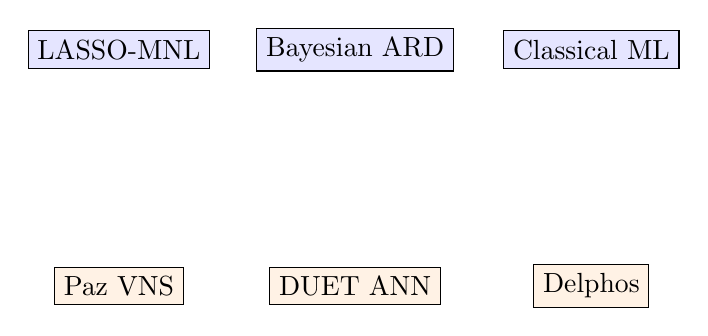
\begin{tikzpicture}[node distance=3cm, auto]
  \node (lasso) [draw, rectangle, fill=blue!10] {LASSO-MNL};
  \node (ard) [draw, rectangle, fill=blue!10, right of=lasso] {Bayesian ARD};
  \node (ml) [draw, rectangle, fill=blue!10, right of=ard] {Classical ML};
  
  \node (paz) [draw, rectangle, fill=orange!10, below of=lasso] {Paz VNS};
  \node (duet) [draw, rectangle, fill=orange!10, below of=ard] {DUET ANN};
  \node (delphos) [draw, rectangle, fill=orange!10, below of=ml] {Delphos};
\end{tikzpicture}
\end{center}

\small
\textbf{Top row}: Classical / Statistical methods for discrete choice specification.
\textbf{Bottom row}: LLM-guided and learned search methods.
\normalsize

%=======================================================================
\section{Related Works}
\label{sec:related}
%=======================================================================

\subsection{Related Work}

\subsubsection{LLM-Guided Program/Equation Search}
\begin{itemize}
\item FunSearch (Romera-Paredes et al., \emph{Nature} 2023); LLM-guided symbolic regression.
\item LLM-SR (Shojaee et al., ICLR 2025); Neural-guided equation discovery.
\item LaSR (Grayeli et al., NeurIPS 2024); Large symbolic regression model.
\item SR-LLM (\emph{PNAS} 2025); Symbolic regression with language models.
\item LLM-SRBench (Shojaee et al., ICML 2025); Symbolic regression benchmark.
\item KeplerAgent (2025); LLM-based scientific discovery agent.
\item PITR (2025); Physical integration with text representations.
\item Physics-informed SR with pretrained LLMs (\emph{Scientific Reports} 2025); Incorporating domain knowledge.
\end{itemize}

\subsubsection{LLM + Evolution / LLM-as-Optimizer}
\begin{itemize}
\item Eureka (Ma et al., ICLR 2024); LLM-driven reward design.
\item EvoPrompt (Guo et al., ICLR 2024); Evolutionary search with LLMs.
\item LLaMEA (2024); Large language model evolutionary algorithm.
\item LLM-FE (Abhyankar et al., 2025); LLM-based feature engineering.
\item Human--LLM Collaborative Feature Engineering (2025); Interactive feature discovery.
\end{itemize}

\subsubsection{Automated Discrete Choice Model Specification}
\begin{itemize}
\item Delphos (Nova, Hess, van Cranenburgh, 2025); Automated discrete choice model optimization.
\item Paz et al.\ VNS (2021); Variable neighborhood search for model specification.
\item Bayesian ARD (Rodrigues et al., 2019); Relevance determination for choice models.
\item DUET (Han et al., 2024); Deep utility estimation for discrete choice.
\end{itemize}

\subsubsection{Neural \& Interpretable Discrete Choice}
\begin{itemize}
\item TasteNet-MNL (Han et al., 2020); Neural preference learning in choice.
\item Combining DCM + NN (Arkoudi et al., 2023); Hybrid econometric-neural models.
\item Neural-embedded DCM (Wang et al., 2022); Neural components in discrete choice.
\item RUM-NN (2025); Random utility maximization with neural networks.
\item Bayesian Deep Learning for DC (2025); Uncertainty quantification in neural choice.
\item Framing DCM as DNN (Wang \& Zhao, 2018); Neural network interpretation of choice.
\item Choice Modelling in the Age of ML (van Cranenburgh et al., 2022); Survey of machine learning in choice.
\item WTP from LLM Subjective Choices (2025); Willingness-to-pay from language model preferences.
\end{itemize}

\subsubsection{Classical DCM Background}
\begin{itemize}
\item Train, \emph{Discrete Choice Methods with Simulation} (2009); Foundational DCM reference.
\item Rossi, Allenby \& McCulloch, \emph{Bayesian Statistics and Marketing} (2005); Bayesian choice modeling.
\item Greene, ``Panel Data Models for Discrete Choice''; Panel econometrics for choice.
\item Akinc \& Vandebroek (2018); Discrete choice in design of experiments.
\end{itemize}

\subsubsection{LLMs in Econometrics}
\begin{itemize}
\item Ludwig, Mullainathan \& Rambachan, NBER 2025; LLMs for economic measurement.
\item The Challenge of Using LLMs to Simulate Human Behavior (2023); Behavioral validity of language models.
\item EconNLI (2024); Economic reasoning in natural language inference.
\end{itemize}


\end{document}
